\documentclass{fank1basedocument}

\usepackage{graphicx}
\usepackage{hyperref}
\usepackage{tabularx}
\usepackage{titlesec}

\settitle{Documentation (Summit)}

\fancyhead[L]{CSSE375}
\fancyhead[R]{Spring 2024-2025}

\begin{document}

\tableofcontents

\addcontentsline{toc}{section}{Setup Information and Installation Instructions}
\section*{Setup Information and Installation Instructions}
This section describes how to install the game and lists prerequisites that must be installed before installing the game.
\subsection*{Prerequisites}
Before installing the game, ensure the following are installed:
\begin{itemize}
	\item Java 11 (\href{https://www.oracle.com/java/technologies/javase/jdk11-archive-downloads.html}{https://www.oracle.com/java/technologies/javase/jdk11-archive-downloads.html})
\end{itemize}
\subsection*{Installation}
This section includes a summary of the installation instructions and a more detailed
section with screenshots.
\subsubsection*{Summary}
To install the game,
\begin{enumerate}
	\item Go to \href{https://github.com/summit2021237/csse375-project/releases}{https://github.com/summit2021237/csse375-project/releases}
	\item Download and extract the zip file for a release
	\item Run the JAR file (\texttt{csse375-project-1.0.jar}) in the zip file to run the game
		\begin{enumerate}
			\item Note: There should be a \texttt{src/main/resources} directory that was extracted with the JAR file
		\end{enumerate}
\end{enumerate}

\pagebreak

\subsubsection*{Instructions with Screenshots}
\begin{enumerate}
	\item Go to \href{https://github.com/summit2021237/csse375-project/releases}{https://github.com/summit2021237/csse375-project/releases}
		\begin{enumerate}
			\item Or from \href{https://github.com/summit2021237/csse375-project}{https://github.com/summit2021237/csse375-project}, click on ``Releases" in the right sidebar
		\end{enumerate}
		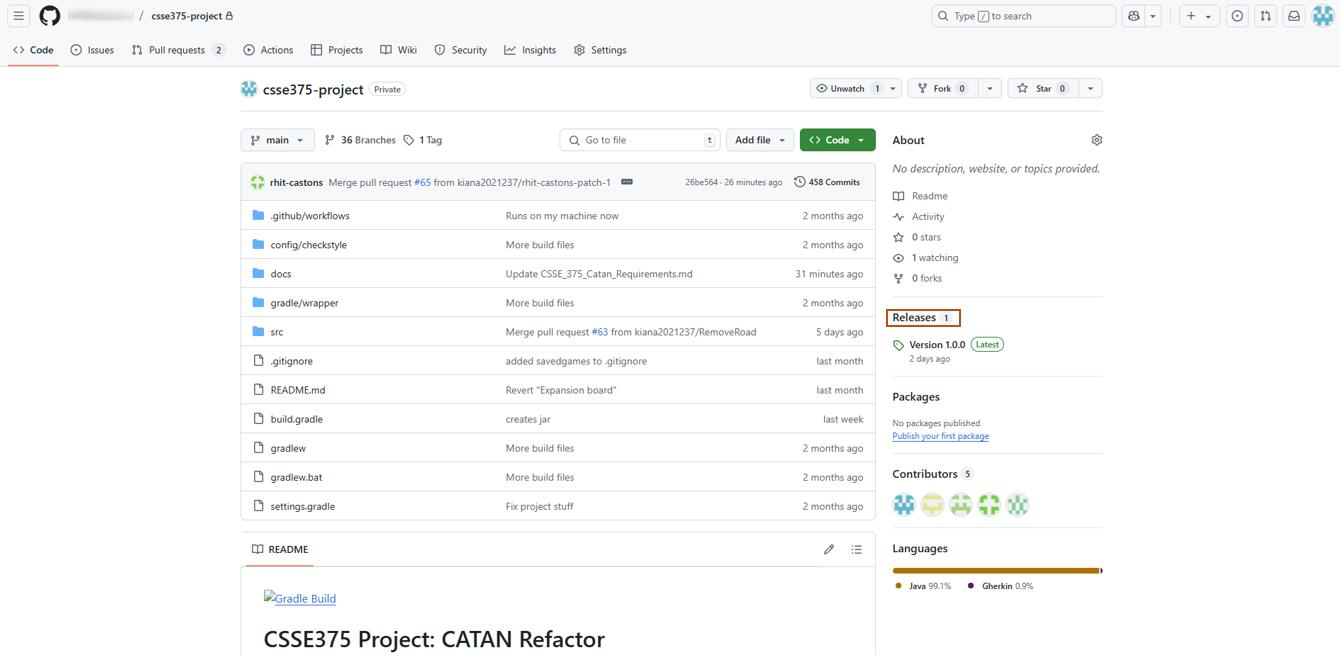
\includegraphics[width=\linewidth]{./images/install01.png}
	\item Click the zip file for the desired version to download it\\
		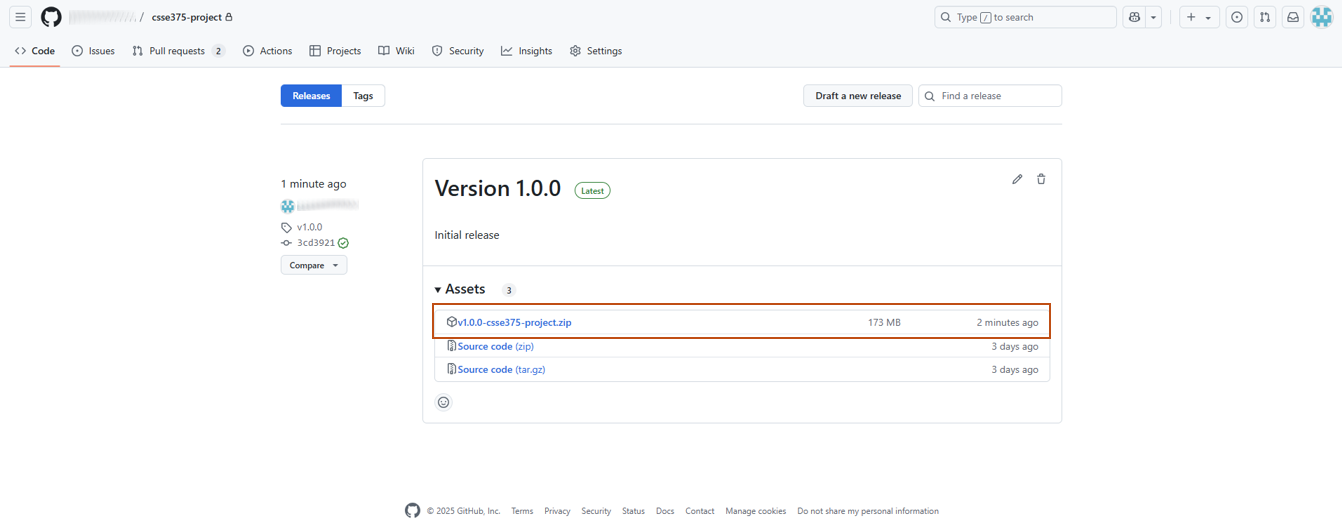
\includegraphics[width=\linewidth]{./images/install02.png}
	\item Extract the files from the zip file

	\pagebreak

	\item Go to the directory that the files were extracted in
		\begin{enumerate}
			\item Note: There should be an \texttt{src/main/resources} directory that was extracted with the JAR file
		\end{enumerate}
		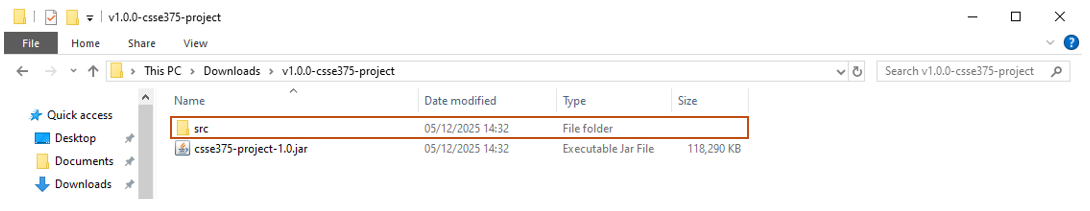
\includegraphics[width=\linewidth]{./images/install03.png}
	\item Double click the JAR file (\texttt{csse375-project-1.0.jar}) to run the game\\
		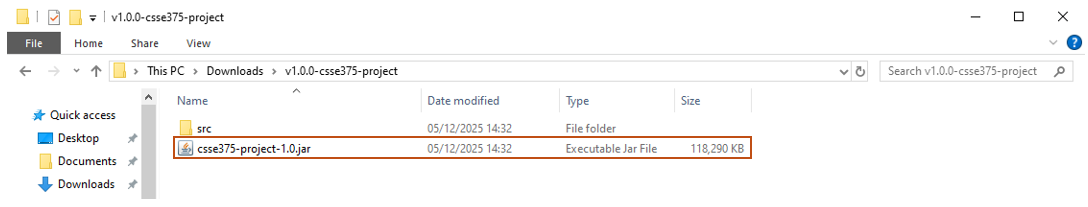
\includegraphics[width=\linewidth]{./images/install04.png}
\end{enumerate}

\addcontentsline{toc}{section}{Development and Maintenance Guide}
\section*{Development and Maintenance Guide}
This guide describes the development environment, programming conventions, configuration management, release process, planned changes, and troubleshooting procedures. It is intended for developers, maintainers, and helpdesk staff.\\

We provide screenshots of installation, configuration, and deployment using IntelliJ, but the user can use any IDE.

\addcontentsline{toc}{subsection}{Development Environment and Continuous Integration Framework}
\subsection*{Development Environment and Continuous Integration Framework}
Catan has a GitHub repository for tracking versions and Gradle as the build tool. The repository has a continuous integration framework using GitHub Actions to run a Gradle build on three different operating systems, ensuring that all the unit tests, integration tests, regression tests, styling checks, and mutation checks pass when creating a pull request to merge into main.

\subsubsection*{Overview}
Repository: \href{https://github.com/summit2021237/csse375-project}{https://github.com/summit2021237/csse375-project}\\
Java: JDK 11\\
JUnit: 5.8.1\\
Gradle: 7.4

\subsubsection*{File Structure}
\begin{tabularx}{\textwidth}{|X|X|}
	\hline
	\texttt{csse375-project/build} & Outputs from Gradle tasks\\
	\hline
	\texttt{csse375-project/config} & Tool configuration files\\
	\hline
	\texttt{csse375-project/docs} & Documentation\\
	\hline
	\texttt{csse375-project/src/main/java} & Source code\\
	\hline
	\texttt{csse375-project/src/main/resources} & Game resources\\
	\hline
	\texttt{csse375-project/src/test/java} & Test files\\
	\hline
	\texttt{csse375-project/src/test/resources} & Test resources\\
	\hline
\end{tabularx}

\subsubsection*{Tools}
\textbf{Gradle:} We use Gradle because that was the build tool that most members of the team were familiar with. The original copy of the game was also set up with Gradle and had tasks for testing and style checks. Gradle has a built-in jar task, which can be configured to create a JAR for release. The build.gradle file is in the top-level directory.\\

\textbf{JUnit:} JUnit is a testing framework that lets developers easily write tests in Java to test Java code.\\

\textbf{Checkstyle:} Checkstyle runs quickly and ensures the formatting in our codebase is consistent for readability and understandability.

\addcontentsline{toc}{subsection}{Set Up Development Environment}
\subsection*{Set Up Development Environment}
To set up the development environment,
\begin{enumerate}
	\item Clone the repository (\href{https://github.com/summit2021237/csse375-project}{https://github.com/summit2021237/csse375-project})
	\item Open the project in an IDE and configure the project and Gradle
\end{enumerate}
With IntelliJ,
\begin{enumerate}
	\item IntelliJ will automatically detect that the project uses Gradle and start a build
	\item Navigate to the Project Structure (under the File menu)
	\item Check that the project uses Java 11
\end{enumerate}
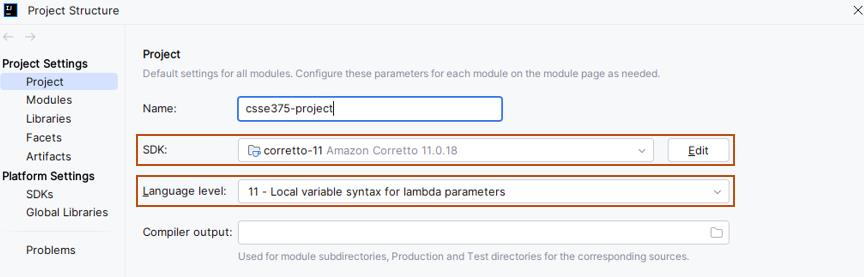
\includegraphics[width=\linewidth]{./images/development01.png}

\addcontentsline{toc}{subsection}{Build Tasks}
\subsection*{Build Tasks}
The following table describes the implemented Gradle build tasks. The most often used tasks are
\begin{itemize}
	\item \texttt{build/build}
	\item \texttt{verification/test}
\end{itemize}
\begin{tabularx}{\textwidth}{|X|X|}
	\hline
	\textbf{Task} & \textbf{Description}\\
	\hline
	\texttt{build/assemble} & Assembles the game\\
	\hline
	\texttt{build/build} & Assembles the game and runs the tests\\
	\hline
	\texttt{build/clean} & Removes the build directory\\
	\hline
	\texttt{other/checkstyleMain} & Runs checkstyle on the production code\\
	\hline
	\texttt{other/checkstyleTest} & Runs checkstyle on the test code\\
	\hline
	\texttt{other/codeCoverageInfo} & Displays summary of code coverage results from jacoco\\
	\hline
	\texttt{reporting/jacocoTestReport} & Generates a code coverage report in the build directory\\
	\hline
	\texttt{verification/check} & Runs all style checks and mutation, unit, integration, and regression tests\\
	\hline
	\texttt{verification/test} & Runs all JUnit tests\\
	\hline
\end{tabularx}

\subsubsection*{Running a Build Task}
In IntelliJ’s Gradle Tool Window, double click the task to run. For example, double click this item to build the game.
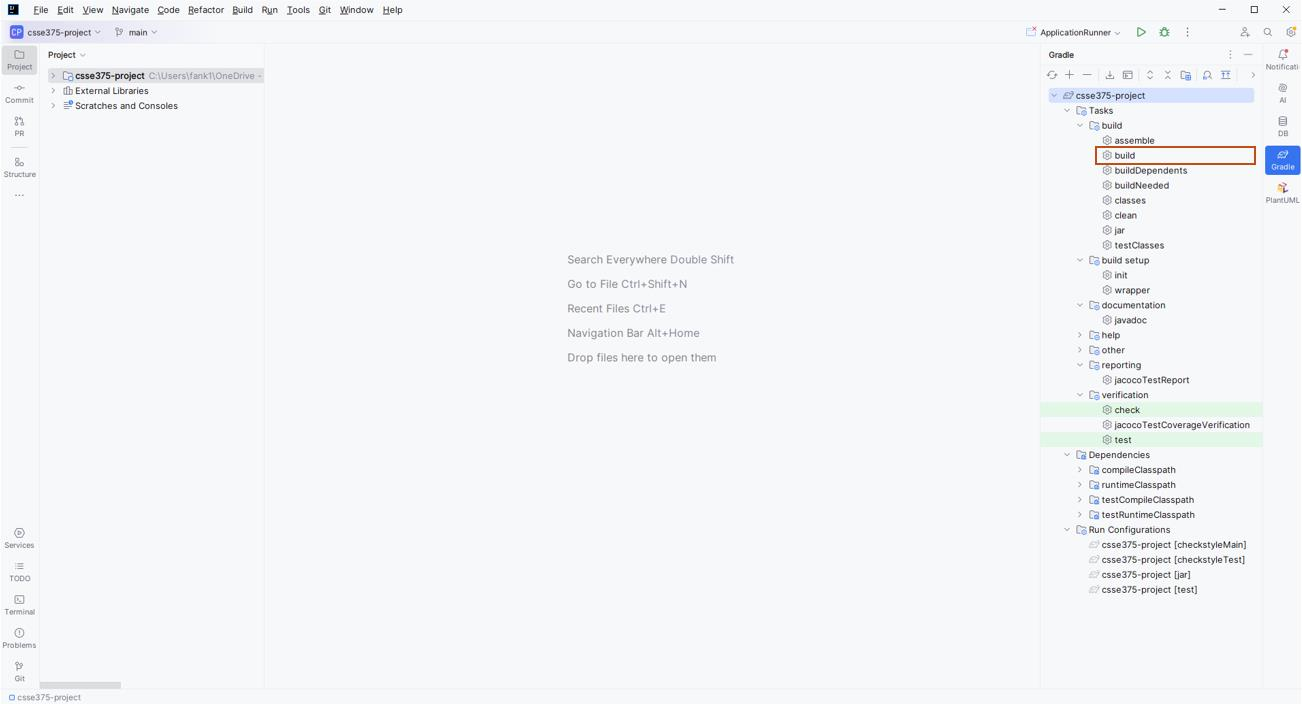
\includegraphics[width=\linewidth]{./images/development02.png}

\addcontentsline{toc}{subsection}{Programming Conventions}
\subsection*{Programming Conventions}
(Written by someone else)

\addcontentsline{toc}{subsection}{Configuration Management}
\subsection*{Configuration Management}
(Written by someone else)

\addcontentsline{toc}{subsection}{Version Numbering}
\subsection*{Version Numbering}
This project uses standard version number conventions, where X.Y.Z is the version with
\begin{itemize}
	\item X: major version number
	\item Y: minor version number
	\item Z: patch number
\end{itemize}

\addcontentsline{toc}{subsection}{Deployment}
\subsection*{Deployment}
This project is deployed by building a JAR file with Gradle and uploading it to the GitHub Releases page. Since the game depends on images, we release a zip file with those images and the JAR.\\

The deployment steps are outlined below.
\begin{enumerate}
	\item Run the \texttt{build/jar} Gradle build task (see Running a Build Task)
	\item The JAR file will be created in \texttt{csse375-project/build/libs} and called \texttt{csse375-project-1.0.jar}\\
		\begin{center}
			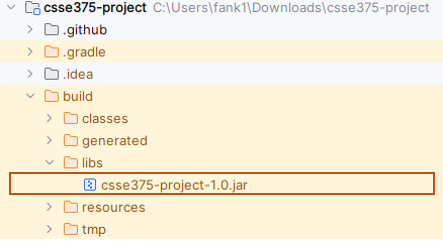
\includegraphics[width=.5\linewidth]{./images/development03.png}
		\end{center}
	\item In the command line, navigate to \texttt{csse375-project/build/libs}
	\item Extract the files from the JAR by running \texttt{jar xf csse375-project-1.0.jar}. The \texttt{csse375-project/build/libs} directory should now contain\\
		\begin{center}
			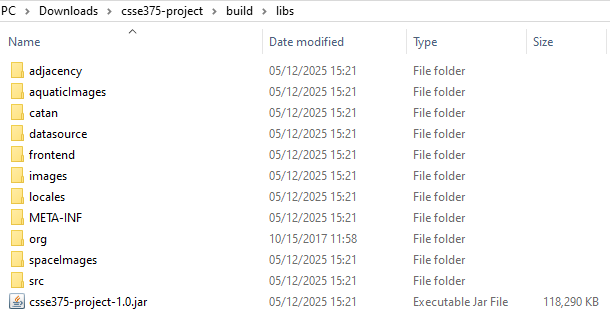
\includegraphics[width=.8\linewidth]{./images/development04.png}
		\end{center}
		\item Delete all the directories except \texttt{src}. The \texttt{csse375-project/build/libs} directory should now contain\\
		\begin{center}
			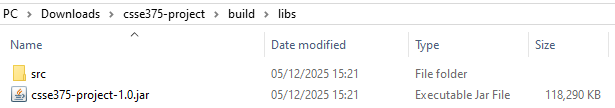
\includegraphics[width=.8\linewidth]{./images/development05.png}
		\end{center}
	\item Rename the JAR to \texttt{v<version>-csse375-project.jar}, where \texttt{<version>} is the version number (see Version Numbering)
	\item Zip
		\begin{itemize}
			\item \texttt{src} directory
			\item \texttt{v<version>-csse375-project.jar}
		\end{itemize}
	\item Rename the zip file to \texttt{v<version>-csse375-project}
	\item Go to \href{https://github.com/summit2021237/csse375-project/releases/}{https://github.com/summit2021237/csse375-project/releases/}
	\item Click the button to draft a new release\\
		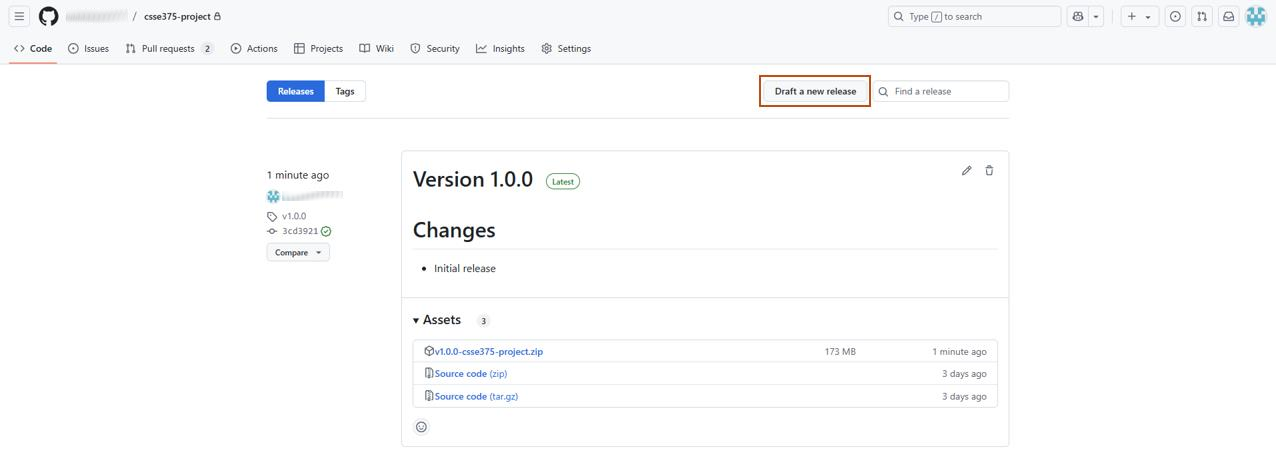
\includegraphics[width=\linewidth]{./images/development06.png}
	\item Enter a name for a new tag for the release version\\
		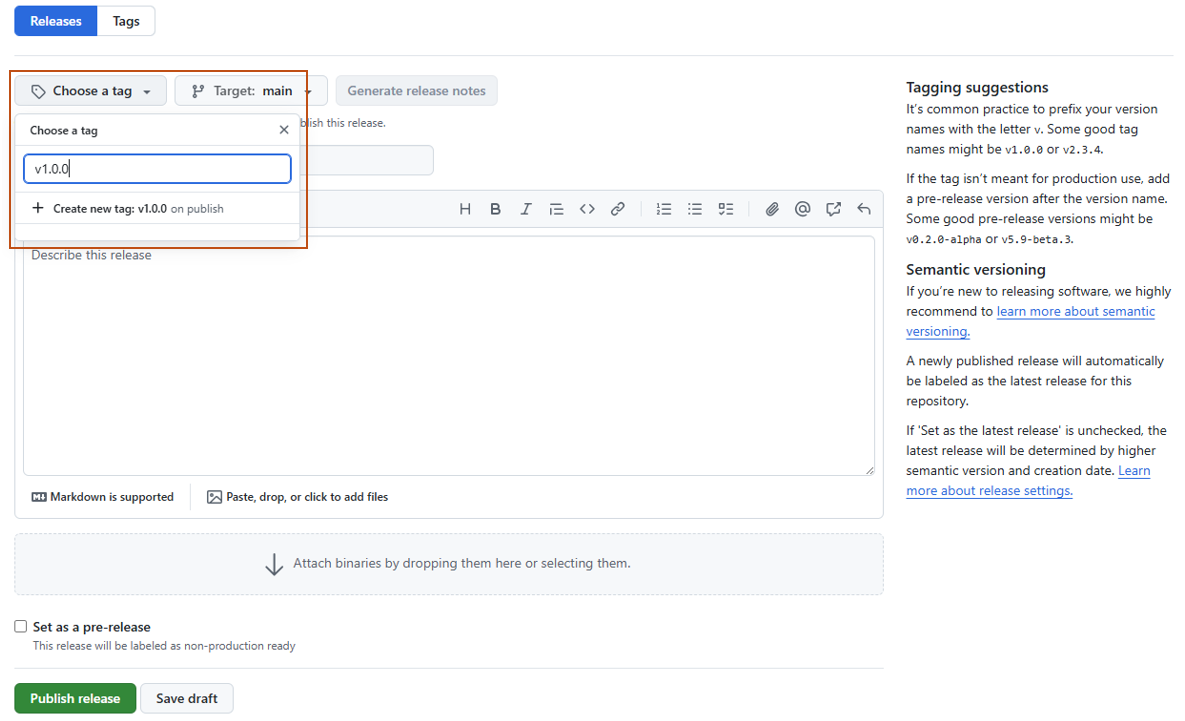
\includegraphics[width=\linewidth]{./images/development07.png}

	\pagebreak

	\item Select the option to create the new tag on publish\\
		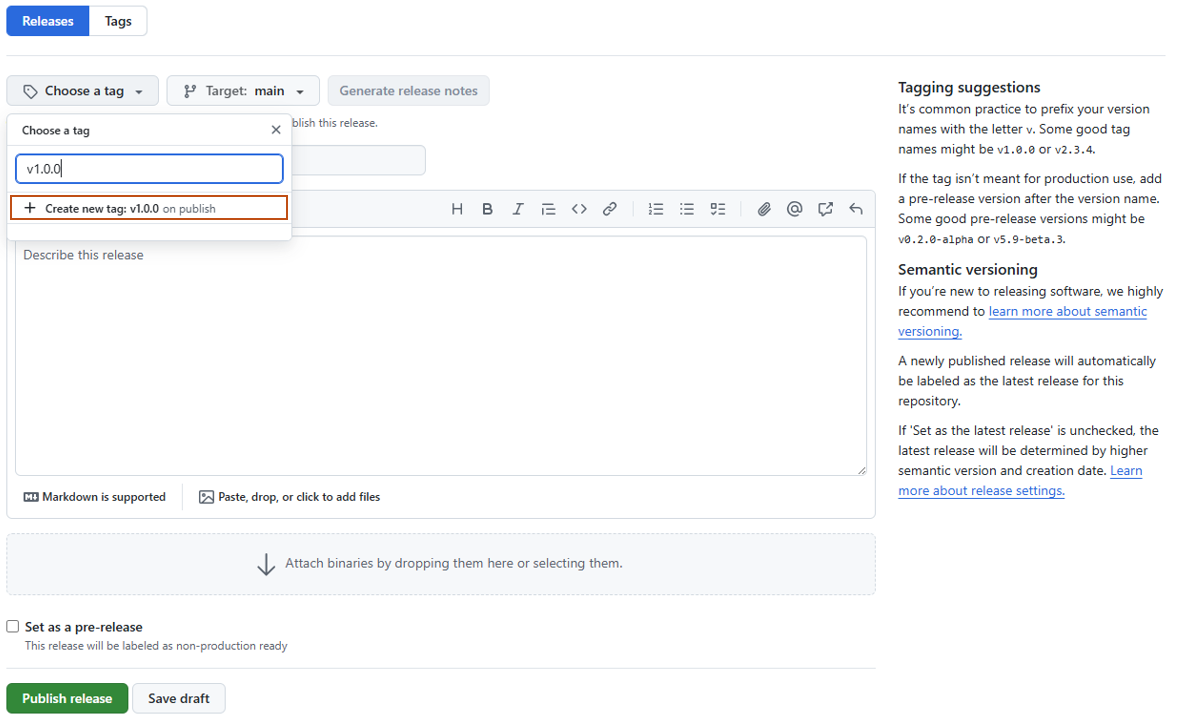
\includegraphics[width=\linewidth]{./images/development08.png}
	\item Set the release title based on the version number\\
		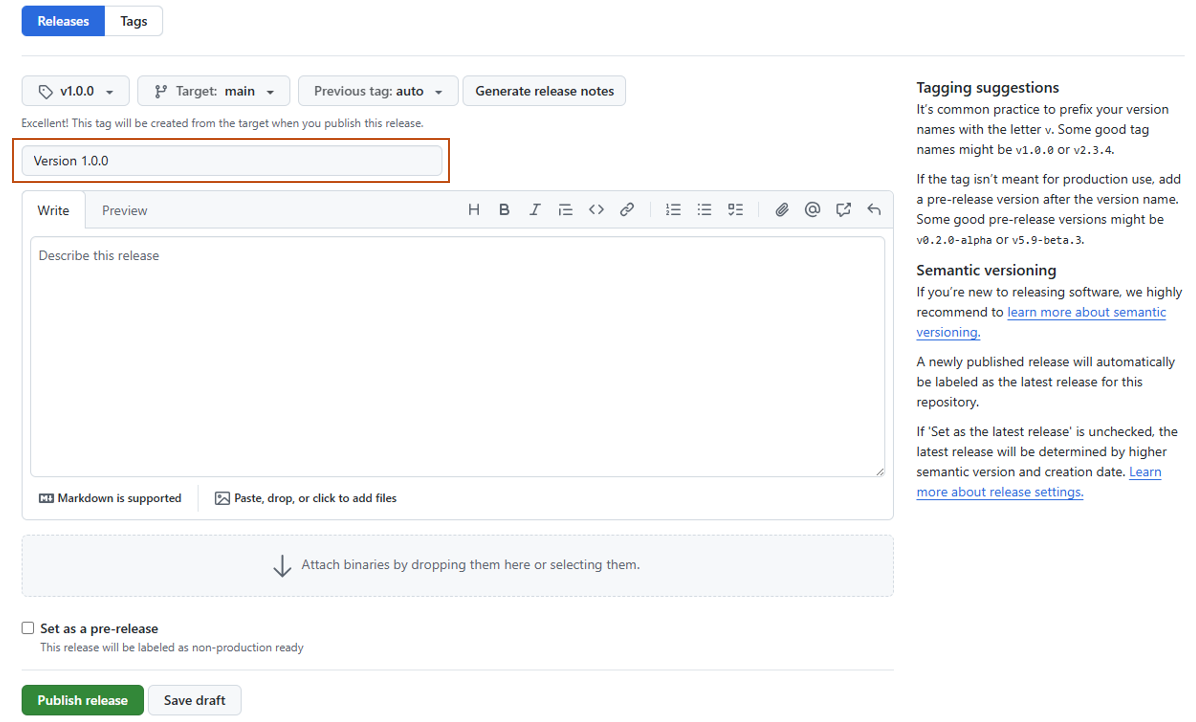
\includegraphics[width=\linewidth]{./images/development09.png}

	\pagebreak

	\item Describe changes made in the release under a change heading\\
		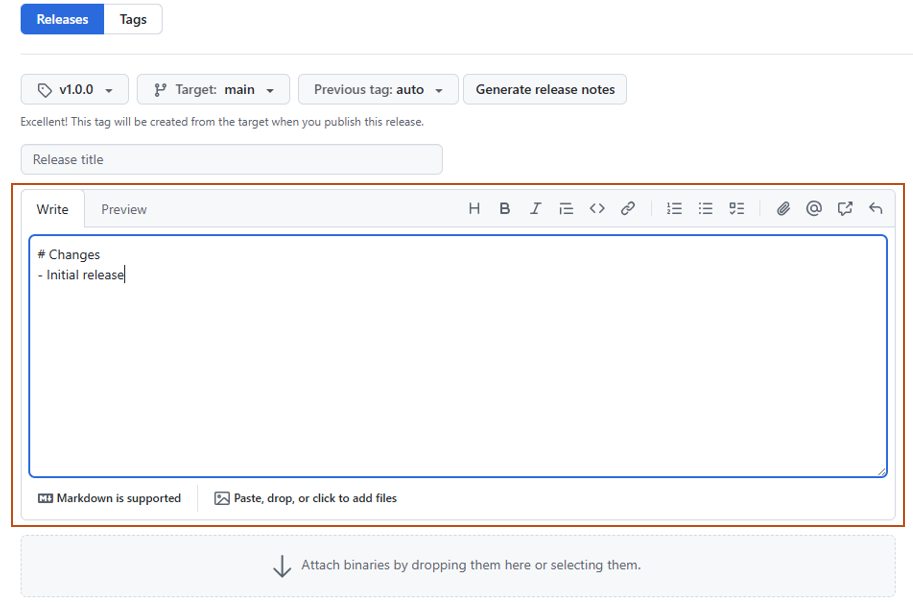
\includegraphics[width=\linewidth]{./images/development10.png}

	\pagebreak

	\item Attach the \texttt{v<version>-csse375-project.zip} file from step 8\\
		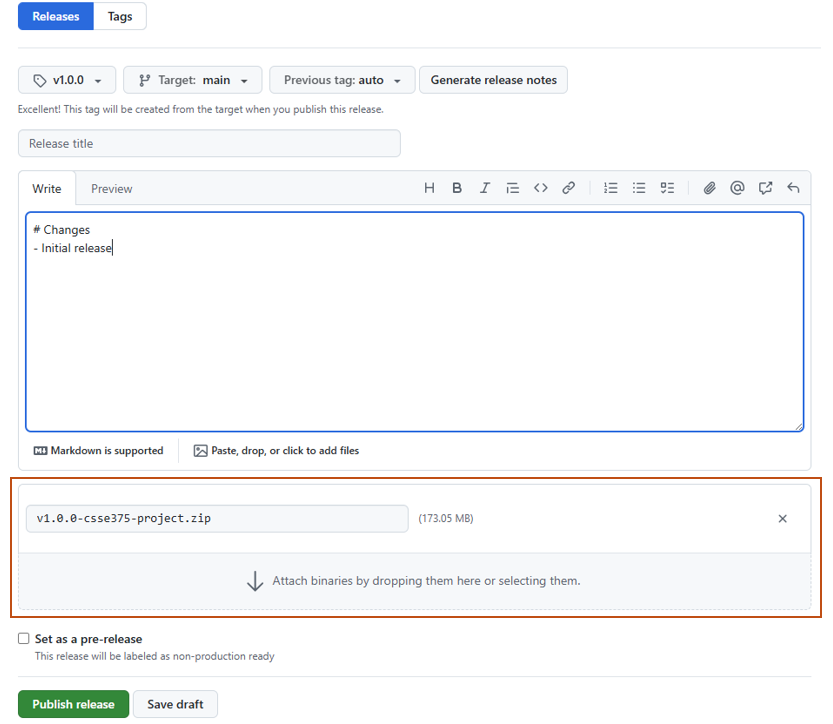
\includegraphics[width=\linewidth]{./images/development11.png}

	\pagebreak

	\item Publish the release\\
		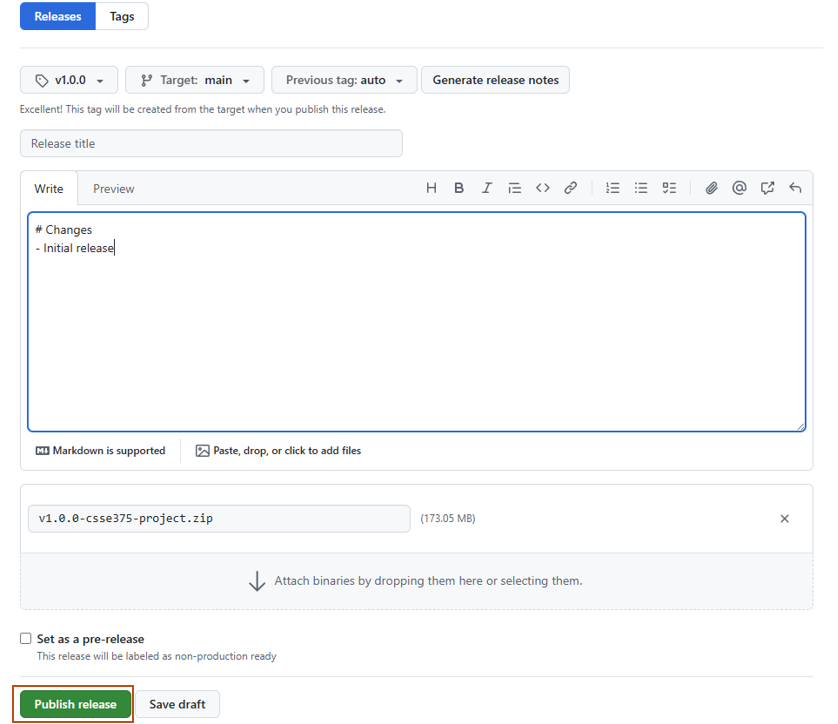
\includegraphics[width=\linewidth]{./images/development12.png}

	\pagebreak

	\item The Releases page should now have the new release\\
		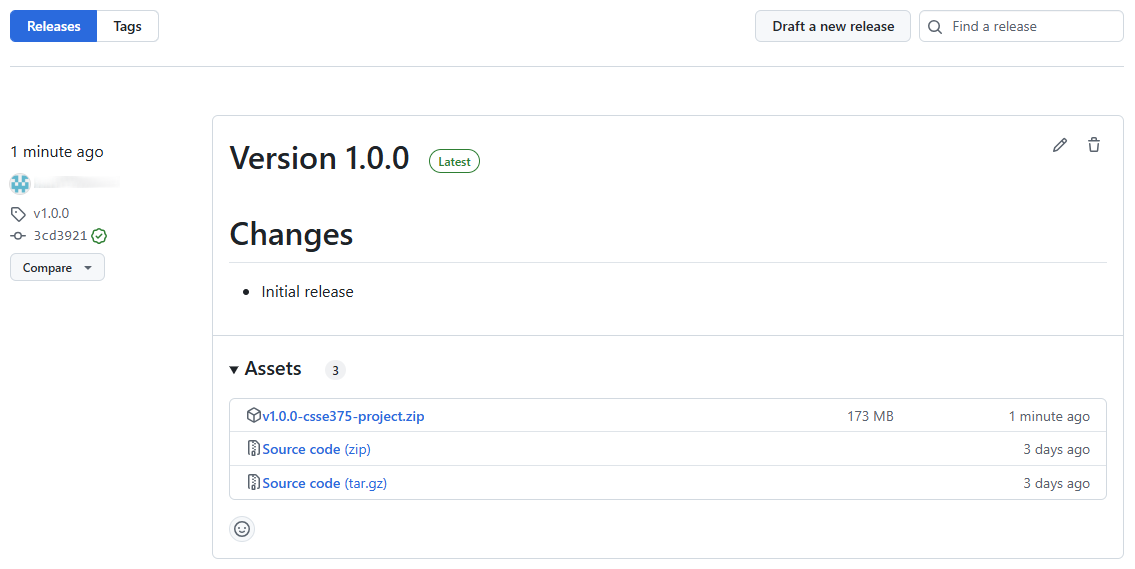
\includegraphics[width=\linewidth]{./images/development13.png}
\end{enumerate}

\addcontentsline{toc}{subsection}{Release Process}
\subsection*{Release Process}
(Written by someone else)

\addcontentsline{toc}{subsection}{Planned Changes}
\subsection*{Planned Changes}
(Written by someone else)

\addcontentsline{toc}{subsection}{Developer Troubleshooting}
\subsection*{Developer Troubleshooting}
(Written by someone else)
\end{document}
